\section{Literature Review} \label{sec:literature}
 
This chapter reviews Deep \acl{mtl} techniques applied to computer vision problems. Emphasis is placed on different types of Deep Multitask architectures and the relevant researches published for each category. Additionally, this chapter includes a historical review of the methods that address the \icao standard, including the methods published on the \fvcongoing website \citep{fvcongoing}. Finally, this chapter is concluded with a discussion around relevant findings of the literature review on both topics.
 
\subsection{Representation Learning}
 
% A similar, but more complex, problem that is closely related to \acs{mtl} is the \acf{ltl}, also known as inductive bias learning or transfer learning \citep{maurer2016benefit}. The main idea behind \acs{ltl} is to learn to perform a new task by exploiting knowledge acquired from previous task experiences. In other words, tasks can ``learn from each other'' by sharing parameters. It has been proposed by \citep{thrun1998learning}, showing that a joint representation that can perform well on training tasks will also generalize to new tasks retrieved from the same ``environment''. Recent studies have also demonstrated dimension-independent bounds \citep{maurer2013sparse, pontil2013excess, pentina2014pac}.
 
% A seminal line of research in the field of \acl{mtl} and Transfer Learning is centered around the concept that tasks are related by means of a shared low-dimensional representation that is jointly learned along with the task parameters \citep{maurer2016benefit}. This approach was first endorsed by the works of \cite{Caruana1997, thrun1998learning, baxter2000model} and later re-examined from a convex optimization and sparsity regularization perspective in \citep{argyriou2006multi}. Representation Learning is also a crucial aspect of \acl{ai}, leading to a renewed interest in the development of nonlinear hierarchical representations through \aclp{dnn}. In the literature, there is a large body of research on Representation Learning, particularly in the fields of \acf{nlp} \citep{Peters2018DeepCW, devlin2018bert, bojanowski2017enriching} and Computer Vision \citep{ren2015faster, krizhevsky2017imagenet}. Since then, interest in \acf{mtrl} has increased, as it is a core component of \acsp{dnn}.
 
According to the literature, Representation Learning approaches can be divided into two main categories: generative and discriminative modeling. Both approaches consider that a helpful representation can explain the variation in data by capturing underlying factors, such as hierarchical relationships, data dependencies, and domain-specific factors. However, there are essential differences in the modeling process, as detailed next.
 
In generative approaches, the representation is learned by modeling the data distribution $p(x)$. In the case of images, it can be the pixels. It presumes that if a helpful model $p(x)$ can create realistic data samples, it must also be able to capture the underlying structure associated with the dependent variable $y$. The conditional distribution $p(y|x)$ can be determined through Bayes' rule and allows the evaluation of discriminative tasks on $y$ \citep{le2020contrastive}. Generally, generative approaches are categorized as unsupervised learning and can be seen, for instance, in the works of \cite{NIPS2014_5ca3e9b1, kingma2013auto}.
 
On the other hand, discriminative approaches learn a representation by directly modeling the conditional distribution $p(y|x)$ through a parametric model. This model takes the data sample $x$ as the input and outputs the label variable $y$. Latent variables $p(v|x)$ are inferred, and downstream decisions $p(y|v)$ are made from these variables. The most applied discriminative approaches are a type of supervised learning (sometimes called ``self-supervised''). Examples of this approach are given in \citep{dosovitskiy2014discriminative, Zhang_2017_CVPR}.
 
Compared to the generative approach, discriminative models present some advantages. Primarily, modeling the distribution of $x$ is computationally intensive and is not essential for extracting representations. Furthermore, the generation process of a generative model can be deemed inefficient if the objective is to obtain a lower-dimensional representation. Lastly, generative models usually employ a more expensive objective function specially designed for the input space.
 
Representation Learning plays an essential role in several fields and applications. First, we highlight \acl{nlp}. It started with the idea of distributed representations for symbolic data introduced by \cite{hinton1986learning}, which was later implemented by \cite{bengio2000neural} in the context of statistical language modeling. In \citep{collobert2011natural}, the authors developed SENNA, a convolutional architecture for sharing representations across different \acs{nlp} tasks, including: part-of-speech tagging, named entity recognition, chunking, semantic role labeling, language modeling, and syntactic parsing. Methods for learning word representations can also be found in the works of \cite{mnih2013learning, pennington2014glove}. Usually, they are based on unsupervised objectives for predicting words or word frequencies from raw text. These methods have demonstrated remarkable achievements when used for transfer learning, overcoming the limitations of supervised models across multiple downstream tasks.
 
In Computer Vision, the most popular methods for image-feature learning are based on \aclp{cnn}. Traditional architectures, such as AlexNet \citep{krizhevsky2017imagenet}, VGG \citep{simonyan2014very}, and ResNet \citep{he2016deep}, are examples of models used for this purpose. They extract hierarchical features learned from input images, which can be later applied to other classifiers such as Neural Networks or SVMs. Additionally, encoder-decoder architectures, like Autoencoders, are well-known learning methods for representation learning. Examples of other Computer Vision models and architectures are presented in the next section.
 
\subsection{Multitask Learning}
 
As discussed in the previous chapter, \acl{mtl} can be defined as a technique to learn multiple tasks \textit{jointly} instead of learning each task independently. It has been studied since the '90s, initially focused on Neural Network models \citep{ thrun1998learning, Caruana1997, baxter2000model}. More recent approaches have been based on structured sparsity and convex optimization \citep{argyriou2006multi} and kernel methods \citep{evgeniou2005learning}.
 
Historically, \acs{mtl} methods have been classified as hard or soft parameter-sharing techniques \citep{vandenhende2021multi}. In hard parameter sharing, initially proposed by \cite{Caruana1997}, network parameters are divided into shared and task-specific parameters. Typically, \acs{mtl} models that use hard parameter sharing contain a shared encoder with task-specific branches \citep{kendall2018multi, chen2018gradnorm, sener2018multi}. As shown by \cite{baxter1997bayesian}, the risk of overfitting in hard parameter sharing is order $N$ smaller than overfitting the task-specific branches, where $N$ is the number of tasks. Intuitively, since it is harder for a model to find a shared representation for all tasks, the probability of overfitting is less likely. On the other hand, in soft parameter sharing, the parameters of each task are handled by a feature-sharing mechanism \citep{ruder2019latent, gao2019nddr, liu2019end}. In this case, each task has a specific model, and the parameters of each model were regularized to be similar. \autoref{fig:mtl_sharing} visually explains the differences between hard and soft parameter sharing.
 
\begin{figure*}[ht]
\centering
\subfigure[Hard Parameter Sharing]{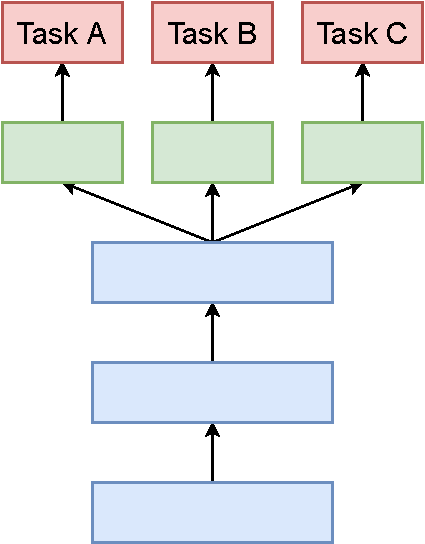
\includegraphics[height=0.35\linewidth]{images/multitask_learning/mtl_hard.pdf}}
\hfill
\subfigure[Soft Parameter Sharing]{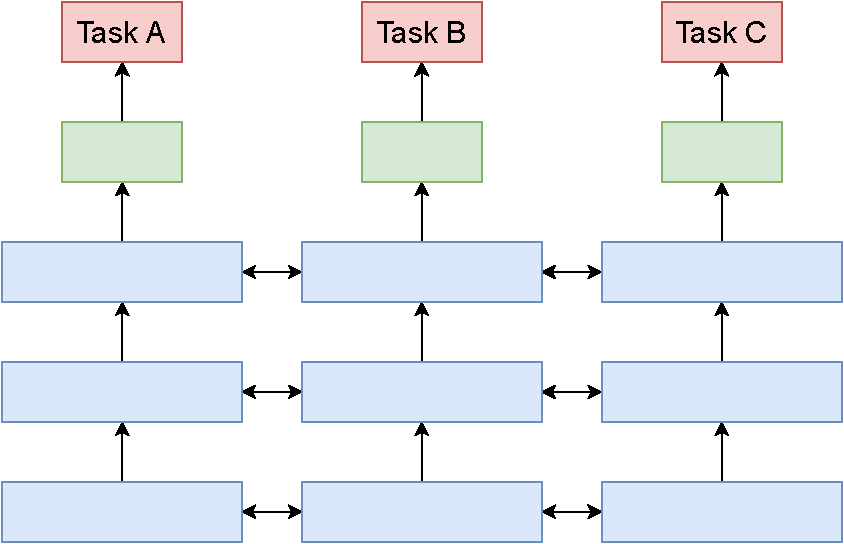
\includegraphics[height=0.35\linewidth]{images/multitask_learning/mtl_soft.pdf}} 
\caption{Types of parameter sharing in \acl{mtl}. The network backbone is represented in blue, whereas the task-specific heads are indicated in green. Source: own elaboration.}
\label{fig:mtl_sharing}
\end{figure*}
 
Various techniques and architectures for \acs{mtl} have been proposed in the literature on Deep Learning. Usually, Deep Multitask Architectures can be divided into encoder-focused and decoder-focused architectures \citep{vandenhende2021multi}. The main characteristic of encoder-focused architectures \citep{kendall2018multi, chen2018gradnorm, sener2018multi} is the presence of an off-the-shelf backbone network, usually called an encoder. The goal of the encoder is to learn a generic representation shared by a set of independent task-specific heads. Differently, the decoder-focused architectures also exchange information during the decoding stage \citep{xu2018pad, zhang2018joint, vandenhende2020mti}. The following subsections discuss the most relevant architectures of Deep \acl{mtl}, according to the above classification.
 
\subsubsection{Encoder-focused Architectures}
 
The \textbf{Cross-stitch networks} \citep{misra2016cross} combine two given activation maps $x_A$ and $x_B$, which belong to tasks $A$ and $B$ respectively, in a learnable linear manner. The transformation can be expressed by learnable weights $\alpha$, as shown in \autoref{eq:cross-stitch}.
 
\begin{equation}
\label{eq:cross-stitch}
\begin{bmatrix}
\bar{x}_A\\ 
\bar{x}_B
\end{bmatrix} = 
\begin{bmatrix}
\alpha_{AA} & \alpha_{AB} \\ 
\alpha_{BA} & \alpha_{BB}
\end{bmatrix}
\begin{bmatrix}
x_A \\ 
x_B
\end{bmatrix}
\end{equation}
 
Each task's $\alpha$ values were initialized in the $[0, 1]$ range and obtained during training through a convex combination. Using this equation, the cross-stitch networks can determine the degree to which the features are shared between different tasks. However, such networks must be pre-trained before stitching them together to maximize performance. Additionally, the size of the Cross-stitch network increases linearly with the number of tasks. 
 
\textbf{Neural Discriminative Dimensionality Reduction CNNs} (NDDR-CNNs) \citep{gao2019nddr} presents a similar architecture with Cross-stitch networks. Nonetheless, a dimensionality reduction component is employed instead of a linear combination to merge all single-task network activations. However, besides the NDDR-CNNs being susceptible to the same problems as the Cross-stitch networks, they also require additional design choices (e.g., where to include the NDDR layers). Nevertheless, NDDR-CNNs and Cross-stitch are limited to local information when the activations from different single-task networks are fused.
 
The \textbf{Multitask Attention Networks} (MTAN) \citep{liu2019end} are an encoder-focused design that combines an encoder with task-specific attention modules in the backbone network. While the encoder is responsible for computing a general pool of features, the task-specific attention module selects features from the public pool by applying a soft attention mask. Regular convolutional layers with sigmoids are used to implement the attention mechanism. Compared to Cross-stitch networks and NDDR-CNNs, the MTAN model is less prone to scalability issues but is also limited to local information to produce the attention mask.
 
\subsubsection{Decoder-focused Architectures}
 
One of the first decoder-focused architectures published in literature was \textbf{PAD-Net} \citep{xu2018pad}. Although the input image is still processed by an off-the-shelf backbone network, the backbone features are further processed by task-specific heads that produce the initial predictions for each task. The task-specific heads contain a per-task feature representation of the input image and are recombined by a multi-modal distillation. The main goal of the distillation unit is to extract the cross-task information using a spatial attention mechanism. The output features $F_k^o$ for a given task $k$ and training sample $i$ are computed according to the \autoref{eq:padnet}:
 
\begin{equation}
\label{eq:padnet}
F_k^o = F_k^i + \sum {\sigma (W_{k,l}F_l^i) \odot F_l^i}
\end{equation}
 
\noindent where $l$ is the feature map index, $W_{k,l}$ is the convolution parameter, $\sigma$ represents a sigmoid function, and $\odot$ denotes element-wise multiplication. However, \autoref{eq:padnet} presumes that task interactions are location-independent. Therefore, there must be no relationship between tasks across the entire image.
 
Similar to PAD-Net, the \textbf{Pattern-Affinitive Propagation Networks} (PAP-Net) \citep{zhang2019pattern} improved multi-model distillation. By statistically observing that pixel affinities contribute to a better alignment with common local structures on the task label space, they proposed leveraging pixel affinities to perform multi-modal distillation. A pixel affinity matrix $M_{T_j}$ is computed by estimating pixel-wise correlations for each task-specific head's features. Then, a cross-task information matrix $\hat{M}_{T_j}$ for each task $T_j$ is learned by an adaptive combination of the affinity matrices $M_{T_j}$ for tasks $T_i$ with learnable weights $\alpha_i^{T_j}$, as defined in \autoref{eq:papnet}:
 
\begin{equation}
\label{eq:papnet}
\hat{M}_{T_j} = \sum_{T_i} {\alpha_i^{T_j} \cdot M_{T_i}}
\end{equation}
 
\noindent
where $i$ represents the index of other tasks. The task features of a task $j$ are refined by the cross-task information matrix $M_{T_j}$. In fact, $M_{T_j}$ is dissipated across the task feature space to spread the pixel correlation for task $T_j$ based on the pixel similarities from the other tasks $T_i$. The learnable weights $\alpha_i^{T_j}$ are obtained by affinity learning layers during the decoding process with different input scales. Unlike the other decoder-focused architectures mentioned, PAP-Net models non-local relationships through pixel similarities computed across the entire image.
 
The \textbf{Joint Task-Recursive Learning} (JTRL), proposed by \cite{zhang2018joint}, recursively predicts two tasks by increasing higher scales to refine the results of past states gradually. Compared to PAD-Net and PAP-Net, there is also a multi-modal mechanism that combines information from earlier task predictions, which are used to refine the later ones. However, the JTRL model can only predict two tasks sequentially and in an intertwined approach. Moreover, the main drawback of the JTRL model is that it is not simple, or even possible, to extend the architecture to more than two tasks because of the intertwined approach to refine predictions.
 
In this thesis, an encoder-focused architecture is applied because there are requirements in the \icao standard that share similar characteristics (e.g., requirements related to the eyes or background). Therefore, the generic representation learned by the encoder may be useful when shared with task-specific heads. Compared with the encoder-focused architectures cited in this chapter, the proposed method does not require pre-training, such as Cross-stitch networks or advanced design choices as in NDDR-CNNs. In addition, the proposed method is easy to scale like MTAN networks. Further details are discussed in Chapter \ref{sec:method}.
 
\subsection{Methods for the \icao Standard}
 
One of the first studies to address ICAO requirements was proposed by \citet{sang2009face}. It presents methods to evaluate the requirements related to illumination conditions and facial poses based on Gabor wavelet features. Furthermore, a method for evaluating image blur is proposed using the Discrete Cosine Transform (DCT). The authors assess their methods using images from the CMU-PIE \citep{sim2002cmu} and FERET \citep{phillips1998feret} datasets. However, only analytical results are presented.
 
The popularization of methods for \icao standard can be credited to the Biolab group from the University of Bologna. In 2009, they presented the Biolab-ICAO framework \citep{maltoni2009biolab}, a benchmark tool for systems assessing face image compliance to ICAO requirements. In 2012, the benchmark was refined, and the official ground-truth face database (4868 images) and testing protocol were presented \citep{ferrara2012face}. In summary, the dataset has 5588 images that were either collected from different sources or artificially generated. A subset of 720 images is publicly provided to the participants, while the 4468 remaining images are private and used to evaluate submitted algorithms. A full description of this dataset is provided in Section \ref{sec:database}. Moreover, the authors proposed BioLabSDK, the first known method published in the literature to evaluate all 23 face-and-pose requirements (8--30 in Table \ref{tab:icao}). BiolabSDK uses different color spaces, a face detector, and points that define the face and its elements to generate a score for each requirement. The paper also compares BioLabSDK against two anonymous SDKs using the \acs{eer} and Rejection Rates. The results can be seen in the first three columns of \autoref{tab:comp}.
 
% Please add the following required packages to your document preamble:
% \usepackage{graphicx}
% \usepackage[table,xcdraw]{xcolor}
% If you use beamer only pass "xcolor=table" option, i.e. \documentclass[xcolor=table]{beamer}
% \usepackage{lscape}
\begin{landscape}
\begin{table*}[tb]
\centering
\caption{Comparison of methods for the pose and photography requirements (8--30) of the \icao standard. The EER and Rejection Rate are presented for each method and were evaluated by the BioLab-ICAO framework in the FICV competition. The "-" indicates the method does not evaluate that requirement or that results were not informed by the authors.}
\label{tab:comp}
\resizebox{\linewidth}{!}{%
\begin{tabular}{rrrrrrrrrrrrrrrrrrrrrrrrr}
\cline{2-25}
 & \multicolumn{2}{c}{\textbf{SDK1}} & \multicolumn{2}{c}{\textbf{SDK2}} & \multicolumn{2}{c}{\textbf{BioLab}} & \multicolumn{2}{c}{\textbf{BioTest}} & \multicolumn{2}{c}{\textbf{BioPass Face}} & \multicolumn{2}{c}{\textbf{id3}} & \multicolumn{2}{c}{\textbf{ICAO SDK}} & \multicolumn{2}{c}{\textbf{FerraraSeg}} & \multicolumn{2}{c}{\textbf{Borges et al.}} & \multicolumn{2}{c}{\textbf{Andrezza et al.}} & \multicolumn{2}{c}{\textbf{Parente et al.}} & \multicolumn{2}{c}{\textbf{HMAX}} \\ \cline{2-25} 
\textbf{Req. \#} & \multicolumn{1}{c}{EER} & \multicolumn{1}{c|}{{\color[HTML]{9B9B9B} Rej.}} & \multicolumn{1}{c}{EER} & \multicolumn{1}{c|}{{\color[HTML]{9B9B9B} Rej.}} & \multicolumn{1}{c}{EER} & \multicolumn{1}{c|}{{\color[HTML]{9B9B9B} Rej.}} & \multicolumn{1}{c}{EER} & \multicolumn{1}{c|}{{\color[HTML]{9B9B9B} Rej.}} & \multicolumn{1}{c}{EER} & \multicolumn{1}{c|}{{\color[HTML]{9B9B9B} Rej.}} & \multicolumn{1}{c}{EER} & \multicolumn{1}{c|}{{\color[HTML]{9B9B9B} Rej.}} & \multicolumn{1}{c}{EER} & \multicolumn{1}{c|}{{\color[HTML]{9B9B9B} Rej.}} & \multicolumn{1}{c}{EER} & \multicolumn{1}{c|}{{\color[HTML]{9B9B9B} Rej.}} & \multicolumn{1}{c}{EER} & \multicolumn{1}{c|}{{\color[HTML]{9B9B9B} Rej.}} & \multicolumn{1}{c}{EER} & \multicolumn{1}{c|}{{\color[HTML]{9B9B9B} Rej.}} & \multicolumn{1}{c}{EER} & \multicolumn{1}{c|}{{\color[HTML]{9B9B9B} Rej.}} & \multicolumn{1}{c}{EER} & \multicolumn{1}{c}{{\color[HTML]{9B9B9B} Rej.}} \\ \cline{2-25} 
\textbf{8} & 26.00 & {\color[HTML]{9B9B9B} 8.90} & 48.10 & {\color[HTML]{9B9B9B} 0.60} & 5.20 & {\color[HTML]{9B9B9B} 0.00} & 30.50 & {\color[HTML]{9B9B9B} 36.00} & 1.60 & {\color[HTML]{9B9B9B} 3.30} & 1.70 & {\color[HTML]{9B9B9B} 0.20} & 48.80 & {\color[HTML]{9B9B9B} 0.00} & \textbf{-} & {\color[HTML]{9B9B9B} \textbf{-}} & \textbf{-} & {\color[HTML]{9B9B9B} \textbf{-}} & \textbf{-} & {\color[HTML]{9B9B9B} \textbf{-}} & \textbf{-} & {\color[HTML]{9B9B9B} \textbf{-}} & \textbf{-} & {\color[HTML]{9B9B9B} \textbf{-}} \\
\textbf{9} & 27.50 & {\color[HTML]{9B9B9B} 7.10} & \textbf{-} & {\color[HTML]{9B9B9B} \textbf{-}} & 20.60 & {\color[HTML]{9B9B9B} 0.00} & 24.20 & {\color[HTML]{9B9B9B} 3.10} & 13.30 & {\color[HTML]{9B9B9B} 3.30} & 15.30 & {\color[HTML]{9B9B9B} 15.80} & 47.50 & {\color[HTML]{9B9B9B} 2.50} & \textbf{-} & {\color[HTML]{9B9B9B} \textbf{-}} & 16.90 & {\color[HTML]{9B9B9B} 1.20} & \textbf{-} & {\color[HTML]{9B9B9B} \textbf{-}} & \textbf{-} & {\color[HTML]{9B9B9B} \textbf{-}} & 10.00 & {\color[HTML]{9B9B9B} 0.16} \\
\textbf{10} & \textbf{-} & {\color[HTML]{9B9B9B} \textbf{-}} & \textbf{-} & {\color[HTML]{9B9B9B} \textbf{-}} & 3.40 & {\color[HTML]{9B9B9B} 1.20} & 3.60 & {\color[HTML]{9B9B9B} 1.40} & 4.80 & {\color[HTML]{9B9B9B} 0.50} & \textbf{-} & {\color[HTML]{9B9B9B} \textbf{-}} & \textbf{-} & {\color[HTML]{9B9B9B} \textbf{-}} & \textbf{-} & {\color[HTML]{9B9B9B} \textbf{-}} & \textbf{-} & {\color[HTML]{9B9B9B} \textbf{-}} & \textbf{-} & {\color[HTML]{9B9B9B} \textbf{-}} & \textbf{-} & {\color[HTML]{9B9B9B} \textbf{-}} & \textbf{-} & {\color[HTML]{9B9B9B} \textbf{-}} \\
\textbf{11} & 18.70 & {\color[HTML]{9B9B9B} 4.80} & 50.00 & {\color[HTML]{9B9B9B} 0.80} & 4.00 & {\color[HTML]{9B9B9B} 0.20} & 5.10 & {\color[HTML]{9B9B9B} 1.70} & 1.90 & {\color[HTML]{9B9B9B} 0.00} & 2.10 & {\color[HTML]{9B9B9B} 0.20} & 50.00 & {\color[HTML]{9B9B9B} 88.8} & \textbf{-} & {\color[HTML]{9B9B9B} \textbf{-}} & \textbf{-} & {\color[HTML]{9B9B9B} \textbf{-}} & 3.70 & {\color[HTML]{9B9B9B} 0.00} & \textbf{-} & {\color[HTML]{9B9B9B} \textbf{-}} & 14.29 & {\color[HTML]{9B9B9B} 0.30} \\
\textbf{12} & \textbf{-} & {\color[HTML]{9B9B9B} \textbf{-}} & 3.10 & {\color[HTML]{9B9B9B} 0.00} & 4.20 & {\color[HTML]{9B9B9B} 0.00} & 4.60 & {\color[HTML]{9B9B9B} 0.20} & 3.10 & {\color[HTML]{9B9B9B} 0.20} & 2.90 & {\color[HTML]{9B9B9B} 0.00} & 27.70 & {\color[HTML]{9B9B9B} 0.00} & \textbf{-} & {\color[HTML]{9B9B9B} \textbf{-}} & \textbf{-} & {\color[HTML]{9B9B9B} \textbf{-}} & \textbf{-} & {\color[HTML]{9B9B9B} \textbf{-}} & \textbf{-} & {\color[HTML]{9B9B9B} \textbf{-}} & \textbf{-} & {\color[HTML]{9B9B9B} \textbf{-}} \\
\textbf{13} & \textbf{-} & {\color[HTML]{9B9B9B} \textbf{-}} & 40.80 & {\color[HTML]{9B9B9B} 0.20} & 9.60 & {\color[HTML]{9B9B9B} 0.00} & 9.20 & {\color[HTML]{9B9B9B} 0.00} & 0.00 & {\color[HTML]{9B9B9B} 0.00} & 0.20 & {\color[HTML]{9B9B9B} 0.00} & \textbf{-} & {\color[HTML]{9B9B9B} \textbf{-}} & \textbf{-} & {\color[HTML]{9B9B9B} \textbf{-}} & \textbf{-} & {\color[HTML]{9B9B9B} \textbf{-}} & \textbf{-} & {\color[HTML]{9B9B9B} \textbf{-}} & \textbf{-} & {\color[HTML]{9B9B9B} \textbf{-}} & \textbf{-} & {\color[HTML]{9B9B9B} \textbf{-}} \\
\textbf{14} & \textbf{-} & {\color[HTML]{9B9B9B} \textbf{-}} & 0.00 & {\color[HTML]{9B9B9B} 0.00} & 1.30 & {\color[HTML]{9B9B9B} 0.00} & 32.40 & {\color[HTML]{9B9B9B} 0.60} & 1.30 & {\color[HTML]{9B9B9B} 0.00} & 0.20 & {\color[HTML]{9B9B9B} 0.40} & \textbf{-} & {\color[HTML]{9B9B9B} \textbf{-}} & \textbf{-} & {\color[HTML]{9B9B9B} \textbf{-}} & \textbf{-} & {\color[HTML]{9B9B9B} \textbf{-}} & \textbf{-} & {\color[HTML]{9B9B9B} \textbf{-}} & 1.70 & {\color[HTML]{9B9B9B} 0.00} & \textbf{-} & {\color[HTML]{9B9B9B} \textbf{-}} \\
\textbf{15} & 50.00 & {\color[HTML]{9B9B9B} 81.90} & \textbf{-} & {\color[HTML]{9B9B9B} \textbf{-}} & 12.80 & {\color[HTML]{9B9B9B} 0.00} & 12.40 & {\color[HTML]{9B9B9B} 4.60} & 13.00 & {\color[HTML]{9B9B9B} 6.30} & \textbf{-} & {\color[HTML]{9B9B9B} \textbf{-}} & \textbf{-} & {\color[HTML]{9B9B9B} \textbf{-}} & 13.87 & {\color[HTML]{9B9B9B} 0.00} & \textbf{-} & {\color[HTML]{9B9B9B} \textbf{-}} & \textbf{-} & {\color[HTML]{9B9B9B} \textbf{-}} & 11.90 & {\color[HTML]{9B9B9B} 3.40} & 25.00 & {\color[HTML]{9B9B9B} 0.00} \\
\textbf{16} & 2.90 & {\color[HTML]{9B9B9B} 3.10} & \textbf{-} & {\color[HTML]{9B9B9B} \textbf{-}} & 4.60 & {\color[HTML]{9B9B9B} 0.00} & 6.70 & {\color[HTML]{9B9B9B} 7.10} & 4.60 & {\color[HTML]{9B9B9B} 4.00} & 0.20 & {\color[HTML]{9B9B9B} 1.00} & \textbf{-} & {\color[HTML]{9B9B9B} \textbf{-}} & \textbf{-} & {\color[HTML]{9B9B9B} \textbf{-}} & 3.80 & {\color[HTML]{9B9B9B} 5.00} & \textbf{-} & {\color[HTML]{9B9B9B} \textbf{-}} & \textbf{-} & {\color[HTML]{9B9B9B} \textbf{-}} & \textbf{-} & {\color[HTML]{9B9B9B} \textbf{-}} \\
\textbf{17} & 7.50 & {\color[HTML]{9B9B9B} 3.30} & 17.90 & {\color[HTML]{9B9B9B} 1.40} & 5.20 & {\color[HTML]{9B9B9B} 0.00} & 3.70 & {\color[HTML]{9B9B9B} 7.90} & 5.20 & {\color[HTML]{9B9B9B} 0.40} & \textbf{-} & {\color[HTML]{9B9B9B} \textbf{-}} & 18.70 & {\color[HTML]{9B9B9B} 1.70} & 6.35 & {\color[HTML]{9B9B9B} 0.40} & \textbf{-} & {\color[HTML]{9B9B9B} \textbf{-}} & \textbf{-} & {\color[HTML]{9B9B9B} \textbf{-}} & \textbf{-} & {\color[HTML]{9B9B9B} \textbf{-}} & \textbf{-} & {\color[HTML]{9B9B9B} \textbf{-}} \\
\textbf{18} & \textbf{-} & {\color[HTML]{9B9B9B} \textbf{-}} & 26.00 & {\color[HTML]{9B9B9B} 2.90} & 12.70 & {\color[HTML]{9B9B9B} 0.20} & 12.60 & {\color[HTML]{9B9B9B} 3.80} & 10.70 & {\color[HTML]{9B9B9B} 1.20} & 9.10 & {\color[HTML]{9B9B9B} 6.90} & \textbf{-} & {\color[HTML]{9B9B9B} \textbf{-}} & \textbf{-} & {\color[HTML]{9B9B9B} \textbf{-}} & \textbf{-} & {\color[HTML]{9B9B9B} \textbf{-}} & \textbf{-} & {\color[HTML]{9B9B9B} \textbf{-}} & \textbf{-} & {\color[HTML]{9B9B9B} \textbf{-}} & 40.82 & {\color[HTML]{9B9B9B} 0.00} \\
\textbf{19} & 5.00 & {\color[HTML]{9B9B9B} 2.70} & 50.00 & {\color[HTML]{9B9B9B} 7.50} & 0.60 & {\color[HTML]{9B9B9B} 0.00} & 1.20 & {\color[HTML]{9B9B9B} 0.40} & 1.40 & {\color[HTML]{9B9B9B} 2.50} & 1.70 & {\color[HTML]{9B9B9B} 0.60} & \textbf{-} & {\color[HTML]{9B9B9B} \textbf{-}} & 0.77 & {\color[HTML]{9B9B9B} 0.00} & \textbf{-} & {\color[HTML]{9B9B9B} \textbf{-}} & 1.30 & {\color[HTML]{9B9B9B} 0.00} & \textbf{-} & {\color[HTML]{9B9B9B} \textbf{-}} & \textbf{-} & {\color[HTML]{9B9B9B} \textbf{-}} \\
\textbf{20} & 5.20 & {\color[HTML]{9B9B9B} 4.50} & 34.20 & {\color[HTML]{9B9B9B} 0.00} & 7.40 & {\color[HTML]{9B9B9B} 0.00} & 10.30 & {\color[HTML]{9B9B9B} 8.40} & 1.70 & {\color[HTML]{9B9B9B} 0.00} & 1.00 & {\color[HTML]{9B9B9B} 2.00} & 48.30 & {\color[HTML]{9B9B9B} 1.70} & \textbf{-} & {\color[HTML]{9B9B9B} \textbf{-}} & 4.00 & {\color[HTML]{9B9B9B} 3.70} & \textbf{-} & {\color[HTML]{9B9B9B} \textbf{-}} & \textbf{-} & {\color[HTML]{9B9B9B} \textbf{-}} & 12.50 & {\color[HTML]{9B9B9B} 0.20} \\
\textbf{21} & \textbf{-} & {\color[HTML]{9B9B9B} \textbf{-}} & \textbf{-} & {\color[HTML]{9B9B9B} \textbf{-}} & 2.30 & {\color[HTML]{9B9B9B} 0.20} & 2.40 & {\color[HTML]{9B9B9B} 7.90} & 5.40 & {\color[HTML]{9B9B9B} 8.40} & \textbf{-} & {\color[HTML]{9B9B9B} \textbf{-}} & 30.00 & {\color[HTML]{9B9B9B} 0.00} & \textbf{-} & {\color[HTML]{9B9B9B} \textbf{-}} & \textbf{-} & {\color[HTML]{9B9B9B} \textbf{-}} & \textbf{-} & {\color[HTML]{9B9B9B} \textbf{-}} & \textbf{-} & {\color[HTML]{9B9B9B} \textbf{-}} & \textbf{-} & {\color[HTML]{9B9B9B} \textbf{-}} \\
\textbf{22} & 36.40 & {\color[HTML]{9B9B9B} 8.10} & \textbf{-} & {\color[HTML]{9B9B9B} \textbf{-}} & 13.10 & {\color[HTML]{9B9B9B} 0.40} & 15.90 & {\color[HTML]{9B9B9B} 19.80} & 9.90 & {\color[HTML]{9B9B9B} 0.60} & 10.50 & {\color[HTML]{9B9B9B} 1.20} & \textbf{-} & {\color[HTML]{9B9B9B} \textbf{-}} & \textbf{-} & {\color[HTML]{9B9B9B} \textbf{-}} & \textbf{-} & {\color[HTML]{9B9B9B} \textbf{-}} & 7.70 & {\color[HTML]{9B9B9B} 2.50} & - & {\color[HTML]{9B9B9B} -} & 13.64 & {\color[HTML]{9B9B9B} 0.40} \\
\textbf{23} & \textbf{-} & {\color[HTML]{9B9B9B} \textbf{-}} & \textbf{-} & {\color[HTML]{9B9B9B} \textbf{-}} & 1.90 & {\color[HTML]{9B9B9B} 0.20} & 2.10 & {\color[HTML]{9B9B9B} 1.20} & 1.80 & {\color[HTML]{9B9B9B} 1.20} & 2.70 & {\color[HTML]{9B9B9B} 20.40} & 50.00 & {\color[HTML]{9B9B9B} 0.00} & \textbf{-} & {\color[HTML]{9B9B9B} \textbf{-}} & \textbf{-} & {\color[HTML]{9B9B9B} \textbf{-}} & \textbf{-} & {\color[HTML]{9B9B9B} \textbf{-}} & \textbf{-} & {\color[HTML]{9B9B9B} \textbf{-}} & \textbf{-} & {\color[HTML]{9B9B9B} \textbf{-}} \\
\textbf{24} & \textbf{-} & {\color[HTML]{9B9B9B} \textbf{-}} & \textbf{-} & {\color[HTML]{9B9B9B} \textbf{-}} & 2.10 & {\color[HTML]{9B9B9B} 0.00} & 2.30 & {\color[HTML]{9B9B9B} 0.00} & 2.70 & {\color[HTML]{9B9B9B} 0.80} & \textbf{-} & {\color[HTML]{9B9B9B} \textbf{-}} & \textbf{-} & {\color[HTML]{9B9B9B} \textbf{-}} & \textbf{-} & {\color[HTML]{9B9B9B} \textbf{-}} & \textbf{-} & {\color[HTML]{9B9B9B} \textbf{-}} & \textbf{-} & {\color[HTML]{9B9B9B} \textbf{-}} & \textbf{-} & {\color[HTML]{9B9B9B} \textbf{-}} & \textbf{-} & {\color[HTML]{9B9B9B} \textbf{-}} \\
\textbf{25} & \textbf{-} & {\color[HTML]{9B9B9B} \textbf{-}} & \textbf{-} & {\color[HTML]{9B9B9B} \textbf{-}} & 5.80 & {\color[HTML]{9B9B9B} 0.00} & 3.30 & {\color[HTML]{9B9B9B} 8.40} & 2.10 & {\color[HTML]{9B9B9B} 12.60} & 1.40 & {\color[HTML]{9B9B9B} 15.80} & \textbf{-} & {\color[HTML]{9B9B9B} \textbf{-}} & \textbf{-} & {\color[HTML]{9B9B9B} \textbf{-}} & \textbf{-} & {\color[HTML]{9B9B9B} \textbf{-}} & \textbf{-} & {\color[HTML]{9B9B9B} \textbf{-}} & \textbf{-} & {\color[HTML]{9B9B9B} \textbf{-}} & 0.00 & {\color[HTML]{9B9B9B} 0.00} \\
\textbf{26} & 50.00 & {\color[HTML]{9B9B9B} 62.30} & \textbf{-} & {\color[HTML]{9B9B9B} \textbf{-}} & 6.30 & {\color[HTML]{9B9B9B} 0.00} & 4.00 & {\color[HTML]{9B9B9B} 31.90} & 10.70 & {\color[HTML]{9B9B9B} 13.80} & 6.60 & {\color[HTML]{9B9B9B} 2.30} & \textbf{-} & {\color[HTML]{9B9B9B} \textbf{-}} & \textbf{-} & {\color[HTML]{9B9B9B} \textbf{-}} & \textbf{-} & {\color[HTML]{9B9B9B} \textbf{-}} & \textbf{-} & {\color[HTML]{9B9B9B} \textbf{-}} & \textbf{-} & {\color[HTML]{9B9B9B} \textbf{-}} & 0.00 & {\color[HTML]{9B9B9B} 0.10} \\
\textbf{27} & \textbf{-} & {\color[HTML]{9B9B9B} \textbf{-}} & \textbf{-} & {\color[HTML]{9B9B9B} \textbf{-}} & 14.00 & {\color[HTML]{9B9B9B} 0.00} & 16.50 & {\color[HTML]{9B9B9B} 21.60} & 9.80 & {\color[HTML]{9B9B9B} 0.40} & 6.80 & {\color[HTML]{9B9B9B} 0.80} & \textbf{-} & {\color[HTML]{9B9B9B} \textbf{-}} & \textbf{-} & {\color[HTML]{9B9B9B} \textbf{-}} & \textbf{-} & {\color[HTML]{9B9B9B} \textbf{-}} & \textbf{-} & {\color[HTML]{9B9B9B} \textbf{-}} & \textbf{-} & {\color[HTML]{9B9B9B} \textbf{-}} & \textbf{-} & {\color[HTML]{9B9B9B} \textbf{-}} \\
\textbf{28} & \textbf{-} & {\color[HTML]{9B9B9B} \textbf{-}} & \textbf{-} & {\color[HTML]{9B9B9B} \textbf{-}} & 2.50 & {\color[HTML]{9B9B9B} 0.00} & 3.70 & {\color[HTML]{9B9B9B} 0.00} & 1.40 & {\color[HTML]{9B9B9B} 4.80} & - & {\color[HTML]{9B9B9B} -} & 50.00 & {\color[HTML]{9B9B9B} 0.00} & \textbf{-} & {\color[HTML]{9B9B9B} \textbf{-}} & \textbf{-} & {\color[HTML]{9B9B9B} \textbf{-}} & \textbf{-} & {\color[HTML]{9B9B9B} \textbf{-}} & 1.20 & {\color[HTML]{9B9B9B} 0.50} & \textbf{-} & {\color[HTML]{9B9B9B} \textbf{-}} \\
\textbf{29} & 3.30 & {\color[HTML]{9B9B9B} 52.10} & \textbf{-} & {\color[HTML]{9B9B9B} \textbf{-}} & 6.20 & {\color[HTML]{9B9B9B} 0.00} & 5.00 & {\color[HTML]{9B9B9B} 2.70} & 3.80 & {\color[HTML]{9B9B9B} 0.00} & 0.60 & {\color[HTML]{9B9B9B} 0.40} & \textbf{-} & {\color[HTML]{9B9B9B} \textbf{-}} & \textbf{-} & {\color[HTML]{9B9B9B} \textbf{-}} & \textbf{-} & {\color[HTML]{9B9B9B} \textbf{-}} & \textbf{-} & {\color[HTML]{9B9B9B} \textbf{-}} & 4.20 & {\color[HTML]{9B9B9B} 0.20} & 10.71 & {\color[HTML]{9B9B9B} 0.40} \\
\textbf{30} & \textbf{-} & {\color[HTML]{9B9B9B} \textbf{-}} & \textbf{-} & {\color[HTML]{9B9B9B} \textbf{-}} & 21.60 & {\color[HTML]{9B9B9B} 0.00} & 15.40 & {\color[HTML]{9B9B9B} 14.20} & 1.20 & {\color[HTML]{9B9B9B} 2.70} & - & {\color[HTML]{9B9B9B} -} & \textbf{-} & {\color[HTML]{9B9B9B} \textbf{-}} & \textbf{-} & {\color[HTML]{9B9B9B} \textbf{-}} & \textbf{-} & {\color[HTML]{9B9B9B} \textbf{-}} & \textbf{-} & {\color[HTML]{9B9B9B} \textbf{-}} & \textbf{-} & {\color[HTML]{9B9B9B} \textbf{-}} & \textbf{-} & {\color[HTML]{9B9B9B} \textbf{-}} \\ \hline
\textbf{mean (\%)} & 21.10 & 21.70 & 30.00 & 8.10 & 7.30 & 0.10 & 9.90 & 8.00 & 4.80 & 2.90 & 3.90 & 4.30 & 41.20 & 10.50 & 7.00 & 0.10 & 8.20 & 3.30 & 4.20 & 0.80 & 4.80 & 1.00 & 14.10 & 0.20 \\
\textbf{median (\%)} & 18.70 & 7.10 & 34.20 & 0.80 & 5.20 & 0.00 & 5.10 & 3.80 & 3.10 & 1.20 & 1.90 & 0.90 & 48.30 & 0.00 & 6.40 & 0.00 & 4.00 & 3.70 & 3.70 & 0.00 & 3.00 & 0.40 & 12.50 & 0.20 \\
\textbf{avg. time (s)} & \textbf{-} & \textbf{-} & \textbf{-} & \textbf{-} & \textbf{-} & \textbf{-} & \multicolumn{2}{c}{8.2} & \multicolumn{2}{c}{2.2} & \multicolumn{2}{c}{1.2} & \multicolumn{2}{c}{4.0} & \textbf{-} & \textbf{-} & \textbf{-} & \textbf{-} & \textbf{-} & \textbf{-} & \textbf{-} & \textbf{-} & \textbf{-} & \textbf{-} \\
\textbf{max. time (s)} & \textbf{-} & \textbf{-} & \textbf{-} & \textbf{-} & \textbf{-} & \textbf{-} & \multicolumn{2}{c}{10.0} & \multicolumn{2}{c}{3.3} & \multicolumn{2}{c}{5.1} & \multicolumn{2}{c}{6.5} & \textbf{-} & \textbf{-} & \textbf{-} & \textbf{-} & \textbf{-} & \textbf{-} & \textbf{-} & \textbf{-} & \textbf{-} & \textbf{-} \\
\textbf{memory (MB)} & \textbf{-} & \textbf{-} & \textbf{-} & \textbf{-} & \textbf{-} & \textbf{-} & \multicolumn{2}{c}{268} & \multicolumn{2}{c}{126} & \multicolumn{2}{c}{334} & \multicolumn{2}{c}{373} & \textbf{-} & \textbf{-} & \textbf{-} & \textbf{-} & \textbf{-} & \textbf{-} & \textbf{-} & \textbf{-} & \textbf{-} & \textbf{-}
\end{tabular}%
}
\end{table*}
\end{landscape}
 
Currently, the Biolab-ICAO framework is used to evaluate algorithms via an online public competition called \acf{ficv}, hosted on the \fvcongoing website \citep{fvcongoing}. The \acs{ficv} is considered the official evaluation tool for \icao standard and is used by all relevant works presented in the literature or commercial products. The photographic and pose requirements are evaluated individually in terms of the EER. All the results presented in Table \ref{tab:comp} and accomplished by the proposed method in this thesis were evaluated using the \acs{ficv}.
 
To date, four algorithms have been published on the \fvcongoing platform: BioTest \citep{fvcBioTest}, BioPass Face \citep{fvcVsoft}, id3 \citep{fvcICAOCompliance}, and ICAO SDK \citep{fvcSeamfix} (see Table \ref{tab:comp}). Compared with BioLabSDK, such algorithms achieve comparable or even better performance rates for particular requirements. However, all of these algorithms are commercial \citep{biometrika, id3, seamfix, vsoft}. Thus, there is no detailed explanation of their methodology in the scientific literature.
 
\cite{ferrara2012multi} present a segmentation method for passport images based on a multi-classifier approach. Using the position, color, texture, and histogram classifiers, the algorithm proposed by the authors classifies and post-processes regions in the face image to segment them into four distinct classes: face, hair, clothes, and background. However, the authors applied the segmentation results to analyze only three ICAO requirements (\hairacrosseyes, \variedbackground, and \flashskin), obtaining EERs of 13.87\%, 6.35\%, and 0.77\%, respectively. This method is named as ``FerraraSeg'' in Table \ref{tab:comp}. Two other face segmentation methods for passport images have been proposed in the literature: \cite{hirzer2009automatic} and \cite{subasic2009expert}. Nonetheless, they did not analyze their results regarding the \icao standard.
 
The work of \citet{nguyen2013automated} proposed a set of normalized metrics for the quantitative conformance testing of ICAO requirements. Their method comprises three main steps: foreground and background segmentation, face detection, and facial feature extraction. Each step takes advantage of the color, intensity, and edge information to compute the scores for a subset of requirements. These metrics were evaluated over a subset of the FERET \citep{phillips1998feret}, GTAV \citep{tarres2012gtav}, and FIePI databases. However, results regarding EER are not presented, which is a common practice of algorithms that assess the \icao requirements in the literature.
 
In \cite{parente2016assessing}, methods for individual evaluation of four requirements were proposed. For the \pixelation requirement, the Canny edge detection method was applied in the eye region, and the Hough Transform was used to detect horizontal and vertical lines. In the case of \hairacrosseyes, both eye regions were preprocessed using classic techniques and compared using an XOR operator. For \veiloverface, the authors computed a score based on the proportion of skin pixels presented in the lower region of the face, using the YCrCb color space. Finally, to assess the \mouthopen requirement, the method analyzes the teeth and lips based on a color-search approach inside the detected mouth. The results for each requirement can be seen in Table \ref{tab:comp}.
 
The requirements \unnaturalskintone, \shadowsacrossface, and \flashskin were evaluated in the work of \citet{andrezza2016facial}. As these requirements are directly related to the skin, the authors developed a custom segmentation method. Each pixel in the face image that falls into a predefined range of the YCrCb color space is marked as skin. To evaluate the \unnaturalskintone, a score was computed based on the proportion of pixels with a natural tone according to the histogram analysis. For \flashskin, a metric is defined based on the binarized image of the Y channel of YCrCB. Similarly, the Z channel of the XYZ color space was analyzed to evaluate the shadows in the face. In Table \ref{tab:comp}, the results are shown in the column named ``Andrezza et al.''.
 
The work of \citet{borges2016analysis} analyzed some of the requirements related to the eyes: \eyesclosed, \redeyes, and \lookingaway. First, an appearance-based method was applied to find the eye corners and estimate the iris center based on the Canny edge detector and Hough Circle Transform. Such information is used in the remaining methods. To detect whether the eyes were closed or open, the authors computed a metric based on eye dimensions and the presence of the sclera. For the evaluation of \redeyes, custom computations are performed on RGB, HSV, and YCrCB to find the ``red'' pixels, and three corresponding binarized images are generated. A score was then computed based on the logical operations combining these images. Finally, to assess the \lookingaway requirement, the authors assumed that the eyes were symmetric and inspected each eye's left and right sides. An OR operation was applied between both sides, and a score was computed based on the proportion of the minimum and maximum sums of white pixels. This method is identified by ``Borges et al.'' in Table \ref{tab:comp}.
 
One of the first studies that employed a \acl{dl}-based method for \icao was presented by \cite{ahmadvand2018estimating}. The authors applied the fine-tuning technique to the VGGFace model \citep{simonyan2014very} to train a new model that assesses the \rollpitchyaw requirement. Six different datasets were employed, with a total of 320,000 images, of which only 12,000 were compliant with the ICAO standard. Cross-entropy was used to optimize the model, and the accuracy was chosen to evaluate the final results. The authors reported 95.5\% and 97.8\% accuracy in the PIE \citep{sim2002cmu} and CSIE Robotic \citep{csie2006database} databases, respectively. The evaluation results according to the \acs{ficv} competition are not mentioned in the paper.
 
The \biolabicao framework is used by \cite{hernandez2019faceqnet} to train a method based on \aclp{cnn}, called FaceQnet. In this case, the framework is applied to label the VGGFace2 dataset \citep{cao2018vggface2}. ResNet-50 \citep{he2016deep} was fine-tuned to return a score representing a numerical quality measure for each input image. The authors analyzed if the score could determine whether an image was suitable for face recognition. However, the authors did not provide results regarding the \acs{ficv} competition and, thus, they are not included in Table \ref{tab:comp}.

A similar work to FaceQnet was presented in \citep{hernandez2022faceqvec}, called FaceQvec. In this paper, the authors developed a set of methods to give a quality score for each requirement of \icao standard plus white noise and expression. \acl{dl} methods were applied for \mouthopen, \eyesclosed, \hairacrosseyes, and \rollpitchyaw requirements. The authors evaluated their method using \acf{roc} curve and Accuracy over two \adhoc datasets labeled by experts with approximately 3500 images. However, as in FaceQnet, the authors do not report results using the \acs{ficv} benchmark.
 
Finally, another recent method for evaluating ICAO requirements was published in 2019 \citep{nourbakhshfacial}. The authors proposed a method based on the Hierarchical Max-pooling (HMAX) model, which consists of a CNN with multiresolution spatial pooling. First, face components were extracted from image patches using the Viola-Jones algorithm \citep{viola2001rapid}. Then, the HMAX model was applied to acquire discriminative signatures. The AR \citep{martinez1998ar} and PUT \citep{kasinski2008put} databases were used to train the model for 9 requirements. In Table \ref{tab:comp}, their results are represented by the ``HMAX'' column.
 
\subsection{Conclusions}
 
From the analysis of the literature on \acl{mtl}, some relevant aspects can be highlighted. First, \acs{mtl} is a relatively new field of study when applied to \acl{dl}. Thus, most research on this topic is still beginning, and some gaps can be filled (e.g., the high \acs{eer} of some requirements or the lack of representative datasets). Second, encoder/decoder-focused architectures present advantages and drawbacks. For example, in encoder-focused architectures, the generic representation learned by the encoder may be valuable when shared with task-specific heads. However, they may fail to capture familiar and different aspects among tasks. On the other hand, decoder-focused architectures also share or exchange information during the decoding stage. It can help improve performance; however, such networks usually assume independent tasks or are limited to the number of tasks they can solve. 
 
In this thesis, an encoder-focused architecture is applied since there are requirements in the \icao standard that share similar characteristics (e.g., requirements related to the eyes or background). Therefore, the features learned by the encoder for specific requirements can be leveraged for task-specific heads. Unlike the encoder-focused architectures mentioned in this chapter, the proposed method eliminates the need for pre-training (as in Cross-stitch networks) or complex design choices like in NDDR-CNNs. In addition, the proposed \methodname is easy to scale as MTAN networks. More details will be discussed in Chapter \ref{sec:method}.
 
Regarding Representation Learning, the proposed method employs both generative and discriminative approaches. The generative approach is present in the unsupervised component responsible for creating realistic data samples, whereas it learns a useful representation (called embeddings) by modeling the input distribution. On the other hand, the same representation is also applied to predict different outputs (i.e., requirements and landmark localization). It allows the creation of a proper shared representation built from errors backpropagated from related tasks, as stated in \citep{zhang2014facial}. Also, a more robust requirement assessment can be achieved through joint learning with heterogeneous but subtly correlated tasks. Again, a detailed explanation of the proposed architecture is provided in Chapter \ref{sec:method}.
 
Concerning the literature on the \icao standard, we can conclude that although many studies have addressed this problem for over a decade, it is still an open challenge. For instance, there are still requirements with EERs greater than 10\% as the best result among all published studies (e.g., \lookingaway and \hairacrosseyes). Another point is that most of the best results for each requirement presented in \autoref{tab:comp} are dominated by private companies such as \cite{biometrika}, \cite{id3}, \cite{seamfix}, and \cite{vsoft}. Therefore, there is no detailed explanation of their methods, and there is a lack of state-of-the-art methods published as open research. In fact, 12 of the best results for all 23 requirements are owned by private companies. Another gap is the low number of single methods that evaluate all requirements. Only three methods (\biolab, \biotest, and \biopass) are designed to evaluate all of them. We believe this is due to the absence of public datasets specialized for the ICAO problem. Finally, we can also conclude that \acl{dl} can be a helpful approach for improving the current results of methods that address ICAO requirements. One example is the HMAX work, which achieved 0.0\% EER in two requirements - \framestooheavy and \framecoveringeyes - with very low rejection rates.
 